\documentclass{article}
\usepackage{graphicx}
\usepackage{amsmath}
\usepackage{graphicx}
\usepackage{fancyhdr}
\usepackage{amsfonts}
\usepackage{listings}
\usepackage{float}
\DeclareGraphicsExtensions{.png}


\title{COSC264 Assignment 1}
\author{Dillon Thorsteinn George 38063248 Carl Kenny 93678486}
\date{}

\pagestyle{fancy}
\lhead{Dillon George 38063248}
\rhead{Carl Kenny 93678486}

\begin{document}

\maketitle{}
\null  % Empty line
\nointerlineskip  % No skip for prev line
\vfill
\let\snewpage \newpage
\let\newpage \relax
\let \newpage \snewpage
\vfill 
\break % page break

\newpage

\section*{Percentage Contribution}
Both partners contributed equally to this assignment.

\section*{Question 1}
The bit error rate was modeled using a Binomial distribution. As the probability of each
bit error is independent of every other bit, and for each transmission the message length($n$)
and from this it follows that a Binomial distribution will accurately model the bit error rate.
The number of 'successes' for this distribution are the number of errors occurring in a message of
length $n$.

The python library Numpy was used to calculate the number of erroneous bits in each transmission.
Numpy.random includes a binomial function, this function draws samples from a Binomial probability
distribution.When $n$ and $p$ are passed into this function the return value simulated the number
of errors in one transmission of a packet.

\section*{Question 2}
The total number of bit errors follows a binomial distribution. Thus the probability of having $m$
bit errors('successes') in a message of length $n$ is given by:
\[
        P(X=m) = {n\choose m} p^m (1-p)^{n-m}
\]
Where $p$ is the probability of a bit error.
And so the probability of having at least one bit error is:
\begin{align*}
        P(X\geq 1) &= 1 - P(X = 0) \\
        &= 1 - {n\choose 0} p^0 (1-p)^{n} \\
                   &= 1 - (1 - p)^{n}
\end{align*}
As required.

\section*{Question 3}
In figure 1, there exists an extreme
contrast between the two $p$ values: 0.01 and 0.001. When the error-bit
probability $p$ = 0.01. The line for $p = 0.001$ is a smooth curve which approaches some asymptote(
in this case the asymptote is $u/v$, which is the case where each packet transmitted only once),
for $p = 0.01$ the line displays a 'sawtooth' pattern but still approaches the same asymptote albeit at a
slower rate. This sawtooth behavior is due to the nature of the threshold value, each time the threshold
increases a sudden 'leap' in efficiency is observed, and after this peak the efficiency gradually decreases
until the next increase in the threshold. The gradual decrease is due to the message size increasing, but with 
the number of correctable errors staying the same. This sawtooth does not occur for $p=0.001$ as the number of
errors have a low probability of reaching thee threshold value for any given value of $u$.


\begin{figure}[H]
    \centering
    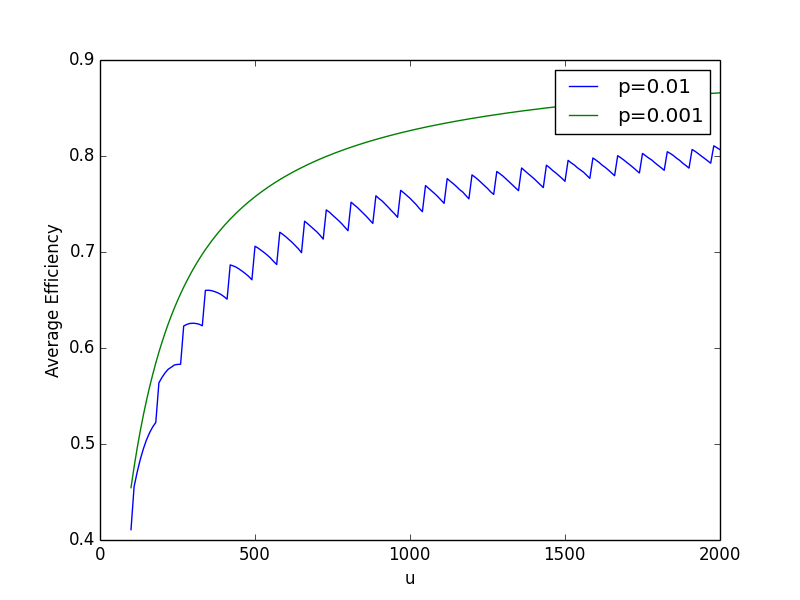
\includegraphics[width=0.8\textwidth]{q3.png}
    \caption{Average efficiency for $p=0.01$, and $p=0.001$ and varying $u$ in the range $[100, 2000]$, where $n-k = \left \lceil{0.1 * (o + u)}\right \rceil$}
    \label{fig:awesome_image}
\end{figure}



\section*{Question 4}
Figure 2. below shows a relatively stable efficiency for $p$ between $0.001$ and around $0.004-0.005$,
after which the efficiency sharply drops. This is due to the lower probabilities on average more bit errors
over the threshold value, and the lower probabilities causing a number of bit errors under the threshold.
This shows that there is a certain range of probabilities for which a binary symmetric channel (BSC)
displays close to no errors, but when a certain threshold is reached the efficiency sharply decreases.

\begin{figure}[H]
    \centering
    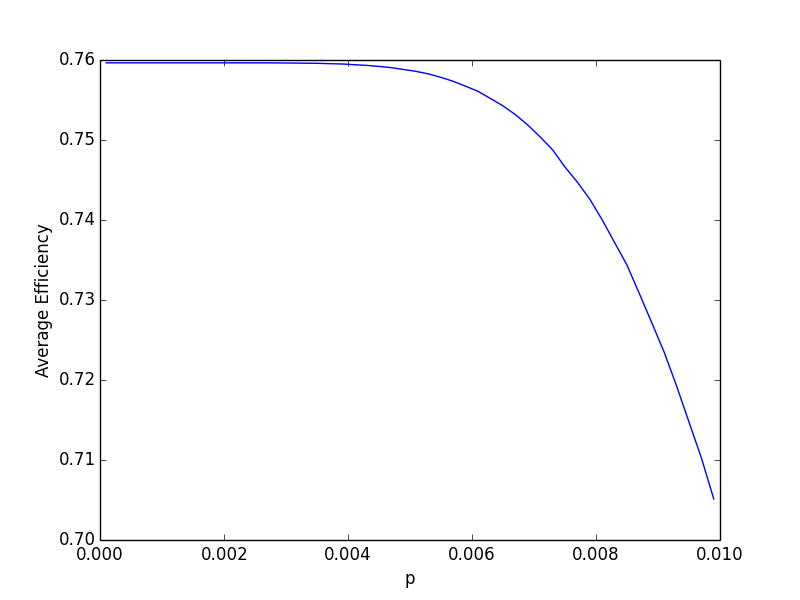
\includegraphics[width=0.8\textwidth]{q4.png}
    \caption{Average efficiency for  $p$ in the range $[0.001, 0.01]$ and fixed $u = 512$, where $n-k = \left \lceil{0.1 * (o + u)}\right \rceil$}
    \label{fig:awesome_image}
\end{figure}



\section*{Question 5}
Figure 3. shows the average efficiency of both a BSC channel and a two-state channel.
Notably both these channels exhibit the same long term behaviour, at  $n-k = 60$ both the
curves overlap and continue to do so for all $n-k$ larger than that. This shows the bit error
rate for the two-state channel averages out to $10^{-3}$ which is identical to that of the BSC channel,
so for a significantly large number of redundant bits a BSC and a two-state channel will behave identically
(if $p_g \approx p_{bsc}$ and $p_g<< p_b$). So the long term behaviour of a two-state channel is determined by $p_b$ in the case where $p_g<< p_b$ as the number of retransmissions when the state is in a bad state will be
much larger than when in a good state, and so the effect of the good state has a negligible effect on the average
efficiency.

When $n-k$ is less than approx. $60$ large jumps can be observed in the average efficiency. When $n-k = 0$ no
bit errors can be corrected so the efficiency is low. Then when $n-k$ is around $20$ the average efficiencies for both channels jumps up, this is due to the threshold being large enough to correct a large majority of the transmissions, this jump is slightly lower for the two-state due to $p_b < p_{bsc}$. And then both channels converge to the same error rate shortly after that.


\begin{figure}[H]
    \centering
    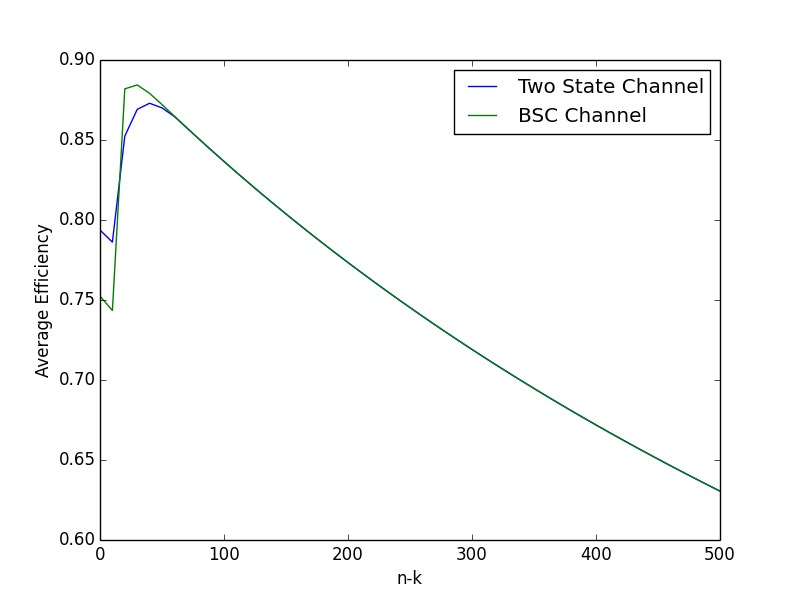
\includegraphics[width=0.8\textwidth]{q5.png}
    \caption{Average efficiency for varying $n-k$ in the range $[0, 500]$ and fixed $u=1024$. For the BSC $p=10^{-3}$.
            For the two-state channel $p_{g} = 10^{-5}$ and $p_b = 1.99*10^{-3}$, $p_{b,b} = p_{g,g} = 0.9$}
    \label{fig:awesome_image}
\end{figure}

\section*{Source Code}

Note: Some errors may have occured when the code was appended to this file. See https://github.com/C-Kenny/264
for source files. To run simulations and plot the figures above run the plot.py file with
the flag -all.

\subsection*{bsc\_channel.py}

\lstinputlisting[language=Python]{bsc_simulation.py}

\subsection*{two\_state\_simulation.py}

\lstinputlisting[language=Python]{two_state_simulation.py}

        \subsection*{hamming.py}

        \lstinputlisting[language=Python]{hamming.py}

        \subsection*{distribution.py}

        \lstinputlisting[language=Python]{distribution.py}

        \subsection*{plot.py}

        \lstinputlisting[language=Python]{plot_CLI.py}
\end{document}
